\chapter{Grundlagen der Künstliche Intelligenz\label{cha:chapter2}}

\section{Künstliche Intelligenz\label{sec:bb}}

Der Begriff künstliche Intelligenz geht auf das Jahr 1956 zurück
und wurde bei einer 
Konferenz in New Hampshire erstmals in der Fachliteratur benutzt. 
Für die Simulierung von Aspekten des 
Lernens, sowie anderer Merkmale der menschlichen Intelligenz von 
Maschinen schlägt der Wissenschaftler John McCarthy den Begriff 
„Künstliche Intelligenz“ vor\footcite{WhatAIBasic}. 


\textit{''Künstliche Intelligenz ist die Fähigkeit einer Maschine, 
menschliche Fähigkeiten wie logisches Denken, Lernen, Planen und 
Kreativität zu imitieren''} \footcite{WasIstKuenstliche2020}\\
ist die heutige Defintion für Künstliche Intelligenz vom Europäischen Parlament 
und deckt sich fast vollständig mit der damaligen Begriffserklärung. Dennoch
bleibt zu sagen, dass es keine einheitliche Definition für den 
Begriff Künstliche Intelligenz gibt und dieser je nach Kontext
unterschiedlich interpretiert werden kann\footcite{WasIstKuenstliche20}.

\subsection{KI-Typen}
KI lässt sich heutzutage in vier KI-Typen unterteilen, 
sowie in schwache und starke künstliche Intelligenz.
\\

Typ 1 KIs sind reaktive 
Maschinen welche eine einzige Aufgabe, für die sie programmiert wurden, 
erfüllen können.
\\

Typ 2 KIs können gesammelte Daten vergangener 
Situationen auf das aktuelle Geschehen anwenden und 
in ihren Entscheidungen berücksichtigen und sind derzeit die gängigste Form von KI.

Typ 3 KIs sind KIs mit starker künstlichen Intelligenz und 
existieren bisher nur in der Theorie. 
Sie können menschliche Emotionen wahrnehmen und ihr Verhalten daran anpassen.

Typ 4 KIs haben eine Selbstwahrnehmung und wissen selber, dass sie denken. 
\footcite{stadlerKuenstlicheIntelligenz}

\subsection{Schwache und starke KI}

Schwache KIs werden für bestimmte Aufgaben eingesetzt und 
können diese meist optimal ausführen. 
Dafür sind sie jedoch auf menschliche Hilfe angewiesen, 
indem Trainingsdaten bereitgestellt und 
Parameter von Lernalgorithmen angepasst werden.

Starke KIs benötigen keine menschliche Eingabe, 
sondern entwickeln sich dadurch nur schneller. 
Sie simulieren keine menschliche Intelligenz, 
sondern entwickeln eigene Intelligenz mit der Zeit. 
Dies ist besonders spannend im Hinblick auf die Frage 
des Urhebers bei Erfindungen, 
da starke KIs ohne vorherige Eingabe Erfindungen entwickeln können.
\footcite{WasIstStarke2023}

Nun stellt sich jedoch die Frage,
welche KIs überhaupt 
Erfindungen erstellen können. Starke KIs sind dazu zwar in 
der Lage, aber bisher nur als theroretisches Konzept verfügbar. 
Deshalb beschränkt sich diese Arbeit zunächst auf schwache KI
mit Erfindungsfähigkeiten. Diese nennt man generative KI 
(generative KI oder generative AI).

\subsection{Generative KI}
Generative KIs
stützen sich auf Deep Learning-Modelle , 
und werden auf großen Datensätzen trainiert, um neue Inhalte zu generieren.  
Sie unterscheiden sich von diskriminativen KI-Modellen, 
die lediglich Daten sortieren und für diese Arbeit aufgrund fehlender
Erschaffungsfähigkeit irrelevant sind. 
Die bekanntesten generativen KI-Anwendungen der letzten Jahre sind
ChatGPT und DALL-E von OpenAI, GitHub CoPilot, Bing Chat von Microsoft, 
Bard von Google, Midjourney, Stable Diffusion und Adobe Firefly \footcite{WasIstGenerative}.

\subsubsection{Deep Learning, neuronale Netze und KI-Modelle}

\paragraph{Deep Learning}
Um Generative KI zu verstehen hilft es Deep Learning zu verstehen.
Beim Deep Learning wird innerhalb eines neuronales Netzes in
mehreren Schichten versucht, 
das Verhalten des menschlichen Gehirns mithilfe von Dateneingaben, 
Gewichtungen und Biases zu simulieren. 
Es gibt die Eingabe und Ausgabeschicht, 
welche allgemein als sichtbare Schichten bezeichnet werden.
Eine Schicht besteht aus Neuronen, welche über Parameter 
mit der nächsten Schicht verbunden sind (Pfeile in \ref{fig:NN}).
Der Parameter Gewichtung bestimmt die Wichtigkeit des Inputs 
zum Neuron in der nächsten Schicht und der Bias die Aktivivierungssensitivität.
In der Eingabeschicht werden die Daten aufgenommen und 
in der Ausgabeschicht der entgültige Output ausgeworfen.
Die Schichten dazwischen werden als verborgene Schichten bezeichnet.
\footcite{WasIstDeep2023}
\footcite{KuenstlicheIntelligenz}
\\
\\
\paragraph{Neuronales Netz}
Ein neuronales Netz (Neural Network) sind die Schichten inklusive ihrer Verbindungen.
Das neuronale Netz wird trainiert indem die Eingabeschicht 
wiederholt mit Daten angereichert wird und diese immer besser klassifiziert.
Der Fortschritt entsteht dabei durch die Neugewichtung der Verbindungen 
zwischen den Schichten. 
In den Schichten werden Muster und Objekte erkannt und zu der vorherigen Schicht
wird eine Vorhersage eingegrenzt oder optimiert 
und Gewichtungen angepasst. 
Das Z in \ref{fig:NN} steht für die lineare Funktion, 
welche diese Vorhersage für die nächste Schicht berechnet.
Dieser Prozess des Berechnens wird als 
Vorwärtspropagierung bezeichnet. 
Entgegen dazu gibt es die Rückwärtspropagierung 
in der Fehler in den Vorhersagen ermittelt werden 
und implizit rückwärts durch die Schichten 
Gewichtungen über eine Loss Function, 
welche die Vorhersagen mit den echten Werten vergleicht, 
angepasst werden. 
Durch Vorwärts- und Rückwärtspropagierung zusammen 
können Vorhersagen getroffen und Fehler korrigiert werden.
\begin{figure}[htb]
    \centering
    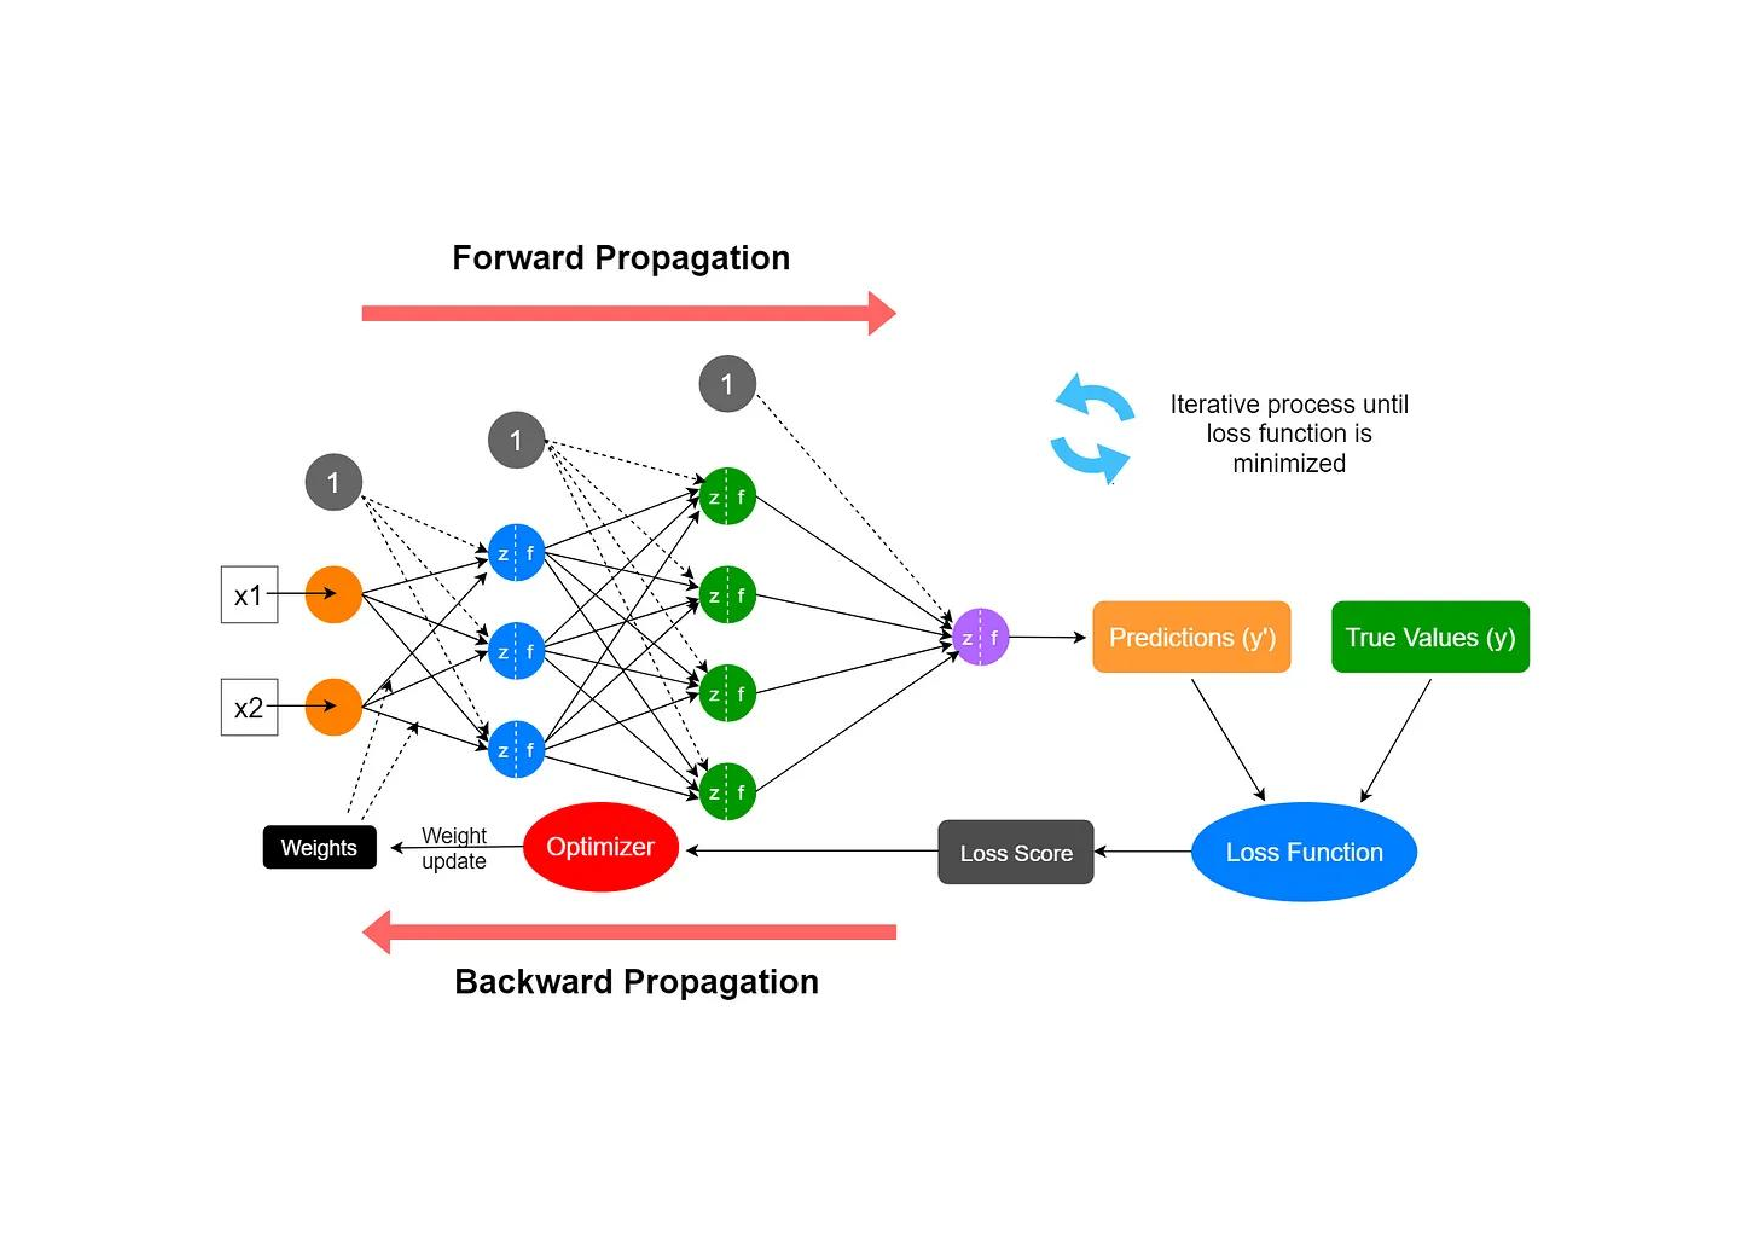
\includegraphics[width=\textwidth]{img/NeuralNetwork.pdf}\\
    \caption{ Neuronales Netz \footcite{pramodithaOverviewNeuralNetwork2022a}}\label{fig:NN}
\end{figure}

  
Dabei unterscheiden sich Neural Networks in 
\gls{CNN} und \gls{RNN}.

CNNs, 
werden in der Erkennung von visuellen Daten eingesetzt, 
da sie Muster erkennen und so Objekte eindeutig identifizieren können.
Dabei werden neue Schichten wie die Konvolutionale Schicht, Pooling-Schicht und
die vollständig verbundene (FC(fully connected)) Schicht eingeführt. 
\footcite{WasSindKonvolutionale2021}

Bei RNNs werden Sequenzen in die Eingabeschicht übergeben, 
wie z.B. Sätze, 
in dem jedes Wort von dem davor und dahinter abhängig ist. 
Dies ist vorallem bei der Identifizierung von natürlicher Sprache 
und umgangssprachlichen Redewendungen nützlich um  
Standardfloskeln identifizieren und nutzen zu können.
\footcite{WasSindRekurrente2023}
Heutige KI-Modelle basieren auf diesen Techniken plus einigen Verbesserungen,
wie \gls{LSTM}, \gls{GRU} 
oder echo state network (ESN).
\\
\\
\paragraph{KI-Modell}
Ein KI-Modell ist das neuronale Netz mit seinen Gewichtungen. 
Vortrainierte Modelle sind z.B. GPT-3 (Generative Pre-trained Transformer Version 3).
\footcite{KuenstlicheIntelligenzKI}
Durch die Eingabe eines Inputs (bei Chat-GPT zumeist Text oder Bild) 
wird ein Output in Bezug auf den Input durch das Modell erzeugt.
\\
\\
Dabei ist wichtig festzuhalten, dass bestehende KIs keine 
eigene Intelligenz besitzen, sondern diese nur simulieren 
und auf Input angewiesen sind. Außerdem sind sie für 
verschiedene Aufgaben spezialisiert und somit als Werkzeug zu sehen. 
Die Entwicklung einer starken KI stellt eine Erschaffung von Intelligenz dar,
welche eigenständig ist und ohne Input Erfindungen erzeugt.

\subsubsection{Genetic Breeding}
Ein weiterer kleiner Teil von generativen KIs ist das Genetic Breeding, 
hier werden evolutionäre Algorithmen genutzt, 
um durch Mutation, Selektion und Rekombination 
neue Algorithmen oder Lösungen zu generieren, 
ähnlich wie in der Natur bei der Evolution von Organismen.
Dieser Prozess ermöglicht es, Lösungen zu entwickeln, 
die nicht explizit von Menschen programmiert wurden, 
sondern sich durch die "Zucht" von Algorithmen 
selbst entwickeln.
Erfindungen die aus Genetic Breeding enstehen werden derzeit
oft als zu generisch und zufällig betrachtet, 
um die Anforderungen an ein Patent zu erfüllen und bieten
derzeit noch zu wenig technische Spezifikationen 
um eine Patentierung zu gewährleisten 
\footcite{hartmannKuenstlicheIntelligenzIm2020}.
Außerdem benötigen auch genetische Algorithmen einen Input
und sind auf die Lösung eines konkreten Problems
ausgelegt. Das Problem wird mit unterschiedlichen
Lösungen gelöst und dann werden die Lösungen bewertet und
die evolutionäre Prozesse beginnen, durch Selektierung, 
Mutation und Rekombination. Diese führen zu weiteren Lösungen,
welche ebenfalls bewertet werden und zu einer nächsten Evolutionsschicht führen.
Eine sog. Fitness-Funktion übernimmt dabei die Bewertung, wie gut das 
Problem durch die einzelnen Lösungen gelöst wurde.

\subsubsection{Zusammenfassung}
Da nun die Grundkonzepte für generative KI definiert sind, ist festzuhalten,
dass die derzeitige KI Input braucht und teilweise auch noch Betreuung während 
des Trainings um Output zu generieren. Es ist derzeit nicht möglich, 
das eine KI ohne eine genaue Problemstellung eine Lösung entwickelt und somit
eigenständig Erfindungen generiert. 
\newpage

